% !TEX TS-program = pdflatex
% !TEX encoding = UTF-8 Unicode

% This is a simple template for a LaTeX document using the "article" class.
% See "book", "report", "letter" for other types of document.

\documentclass[8pt]{article} % use larger type; default would be 10pt

\usepackage[utf8]{inputenc} % set input encoding (not needed with XeLaTeX)
\usepackage{bchart}
\usepackage{longtable}
\usepackage{pgfgantt}
\usepackage{calendar} % Use the calendar.sty style
\usepackage{calc}
\usepackage{ifthen}
\usepackage{tkz-base}
\usepackage{hyperref}
\usepackage{pdfpages}
%%% Examples of Article customizations
% These packages are optional, depending whether you want the features they provide.
% See the LaTeX Companion or other references for full information.

\usepackage{textcomp}
%\usepackage{hyperref}

%%% PAGE DIMENSIONS
\usepackage{geometry} % to change the page dimensions
\geometry{a4paper} % or letterpaper (US) or a5paper or....
% \geometry{margin=2in} % for example, change the margins to 2 inches all round
\geometry{landscape} % set up the page for landscape
%   read geometry.pdf for detailed page layout information

\usepackage{graphicx} % support the \includegraphics command and options

% \usepackage[parfill]{parskip} % Activate to begin paragraphs with an empty line rather than an indent

%%% PACKAGES
\usepackage{booktabs} % for much better looking tables
\usepackage{array} % for better arrays (eg matrices) in maths
\usepackage{paralist} % very flexible & customisable lists (eg. enumerate/itemize, etc.)
\usepackage{verbatim} % adds environment for commenting out blocks of text & for better verbatim
\usepackage{subfig} % make it possible to include more than one captioned figure/table in a single float
% These packages are all incorporated in the memoir class to one degree or another...

%%% HEADERS & FOOTERS
\usepackage{fancyhdr} % This should be set AFTER setting up the page geometry
\pagestyle{fancy} % options: empty , plain , fancy
\renewcommand{\headrulewidth}{0pt} % customise the layout...
\lhead{}\chead{}\rhead{}
\lfoot{}\cfoot{\thepage}\rfoot{}

%%% SECTION TITLE APPEARANCE
\usepackage{sectsty}
\allsectionsfont{\sffamily\mdseries\upshape} % (See the fntguide.pdf for font help)
% (This matches ConTeXt defaults)

%%% ToC (table of contents) APPEARANCE
\usepackage[nottoc,notlof,notlot]{tocbibind} % Put the bibliography in the ToC
\usepackage[titles,subfigure]{tocloft} % Alter the style of the Table of Contents
\renewcommand{\cftsecfont}{\rmfamily\mdseries\upshape}
\renewcommand{\cftsecpagefont}{\rmfamily\mdseries\upshape} % No bold!

%%% END Article customizations

%%% The "real" document content comes below...

%{\footnotesize
%Ce n'est pas parceque les choses sont difficiles que nous n'osons pas, c'est parceque nous n'osons pas qu'elles sont difficiles.
%}
%\makebox[2\width]{hello}

\newcounter{a}
\newcounter{b}

%----------------------------------------------------------
\newcommand{\slice}[4]{
  \pgfmathparse{0.5*#1+0.5*#2}
  \let\midangle\pgfmathresult

   slice
  \draw[thick,fill=black!10] (0,0) -- (#1:1) arc (#1:#2:1) -- cycle;

   outer label
  \node[label=\midangle:#4] at (\midangle:1) {};

   inner label
  \pgfmathparse{min((#2-#1-10)/110*(-0.3),0)}
  \let\temp\pgfmathresult
  \pgfmathparse{max(\temp,-0.5) + 0.8}
  \let\innerpos\pgfmathresult
  \node at (\midangle:\innerpos) {#3};
}

%\subsubsection{Circulatin Graph}
%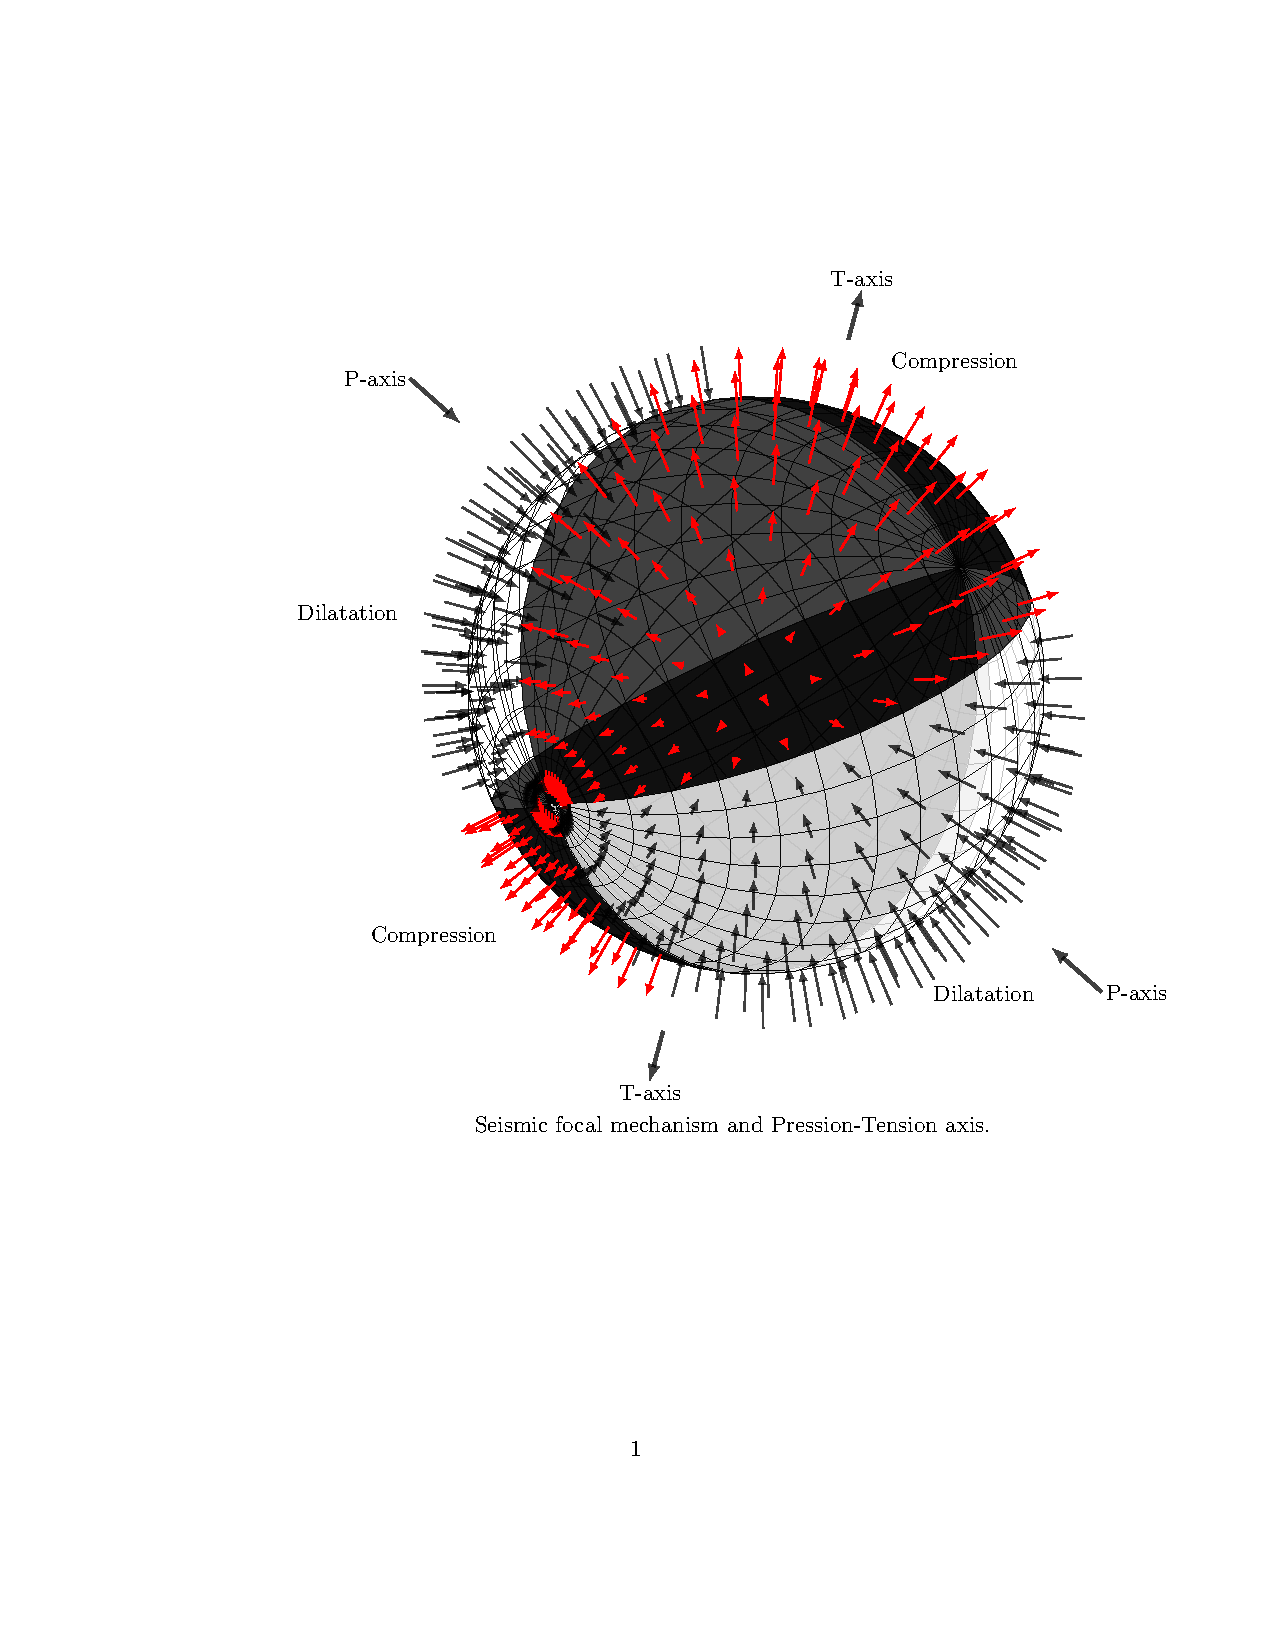
\includegraphics[width=120mm]{SeismicSphere.pdf}
%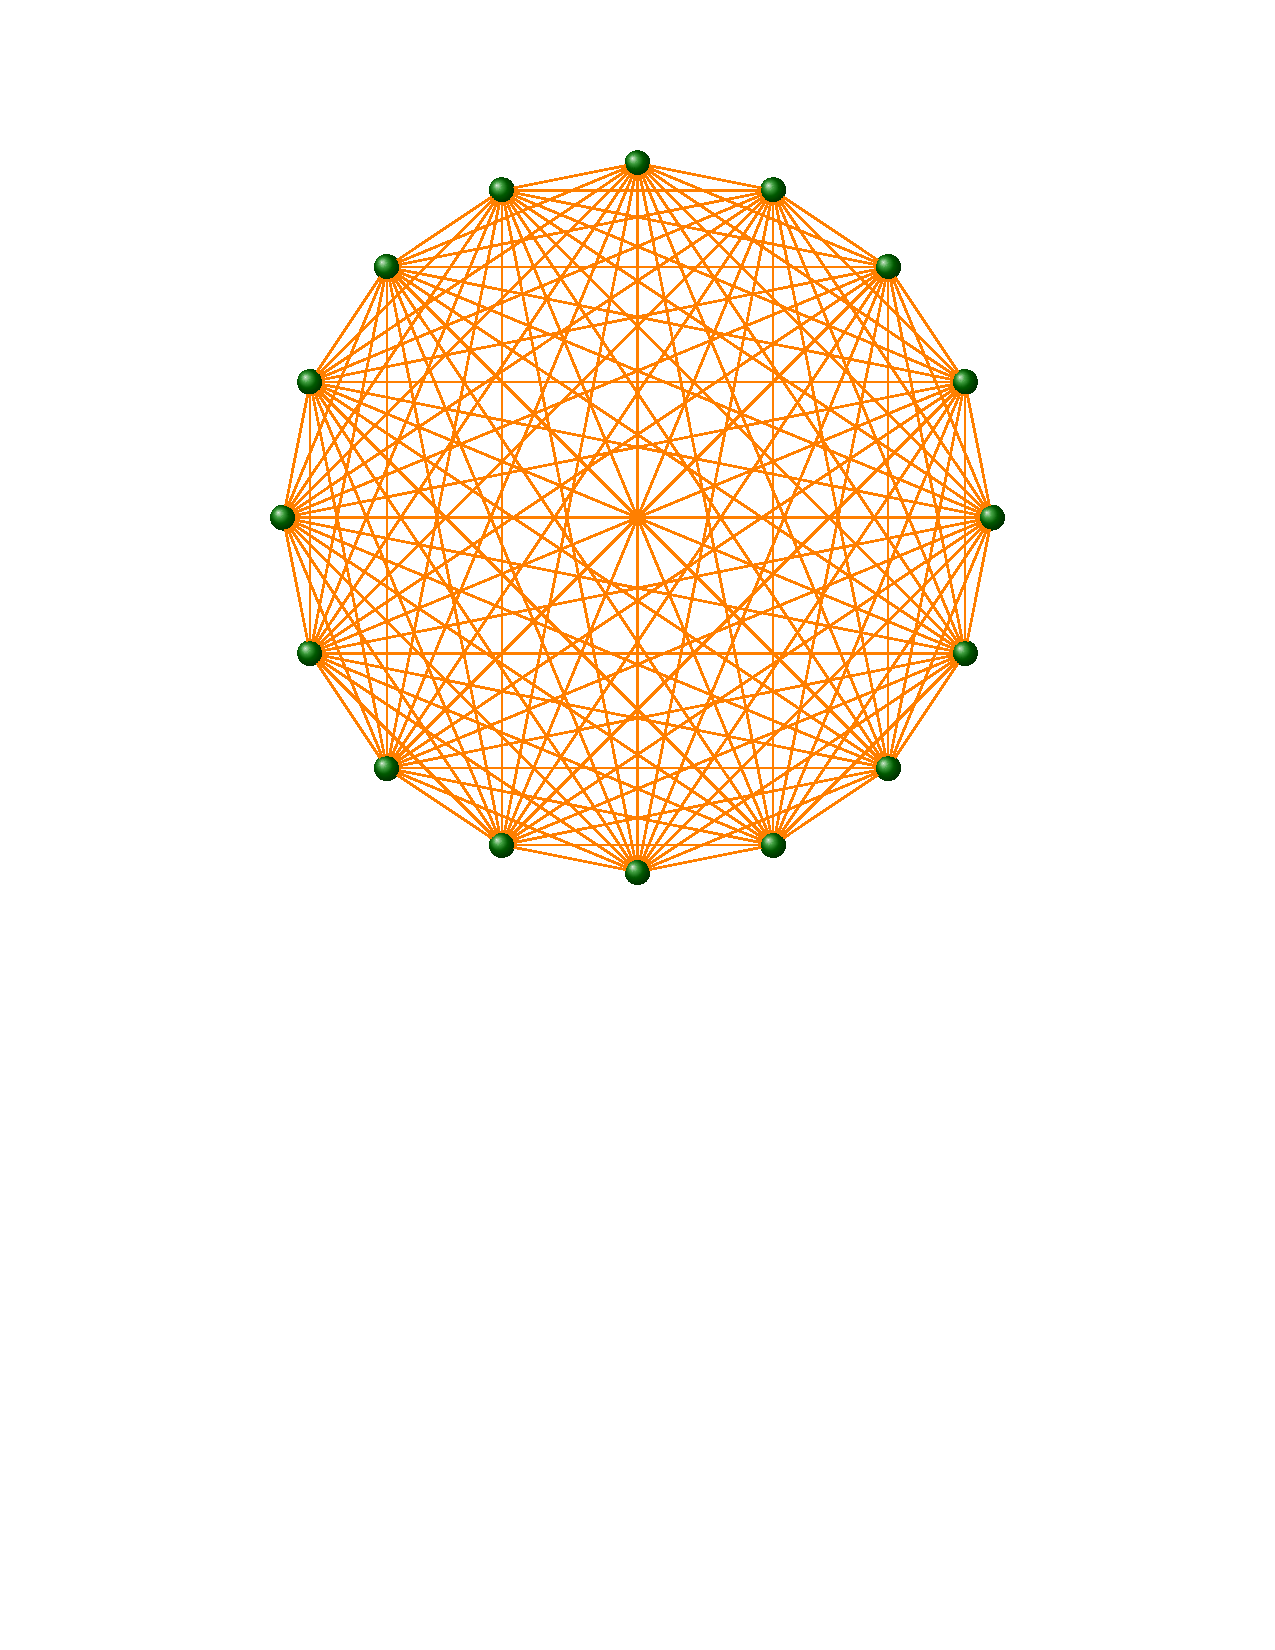
\includepdf[width=50mm]{Circulating-Graph.pdf}

%\subsubsection{Magnetic fields}
%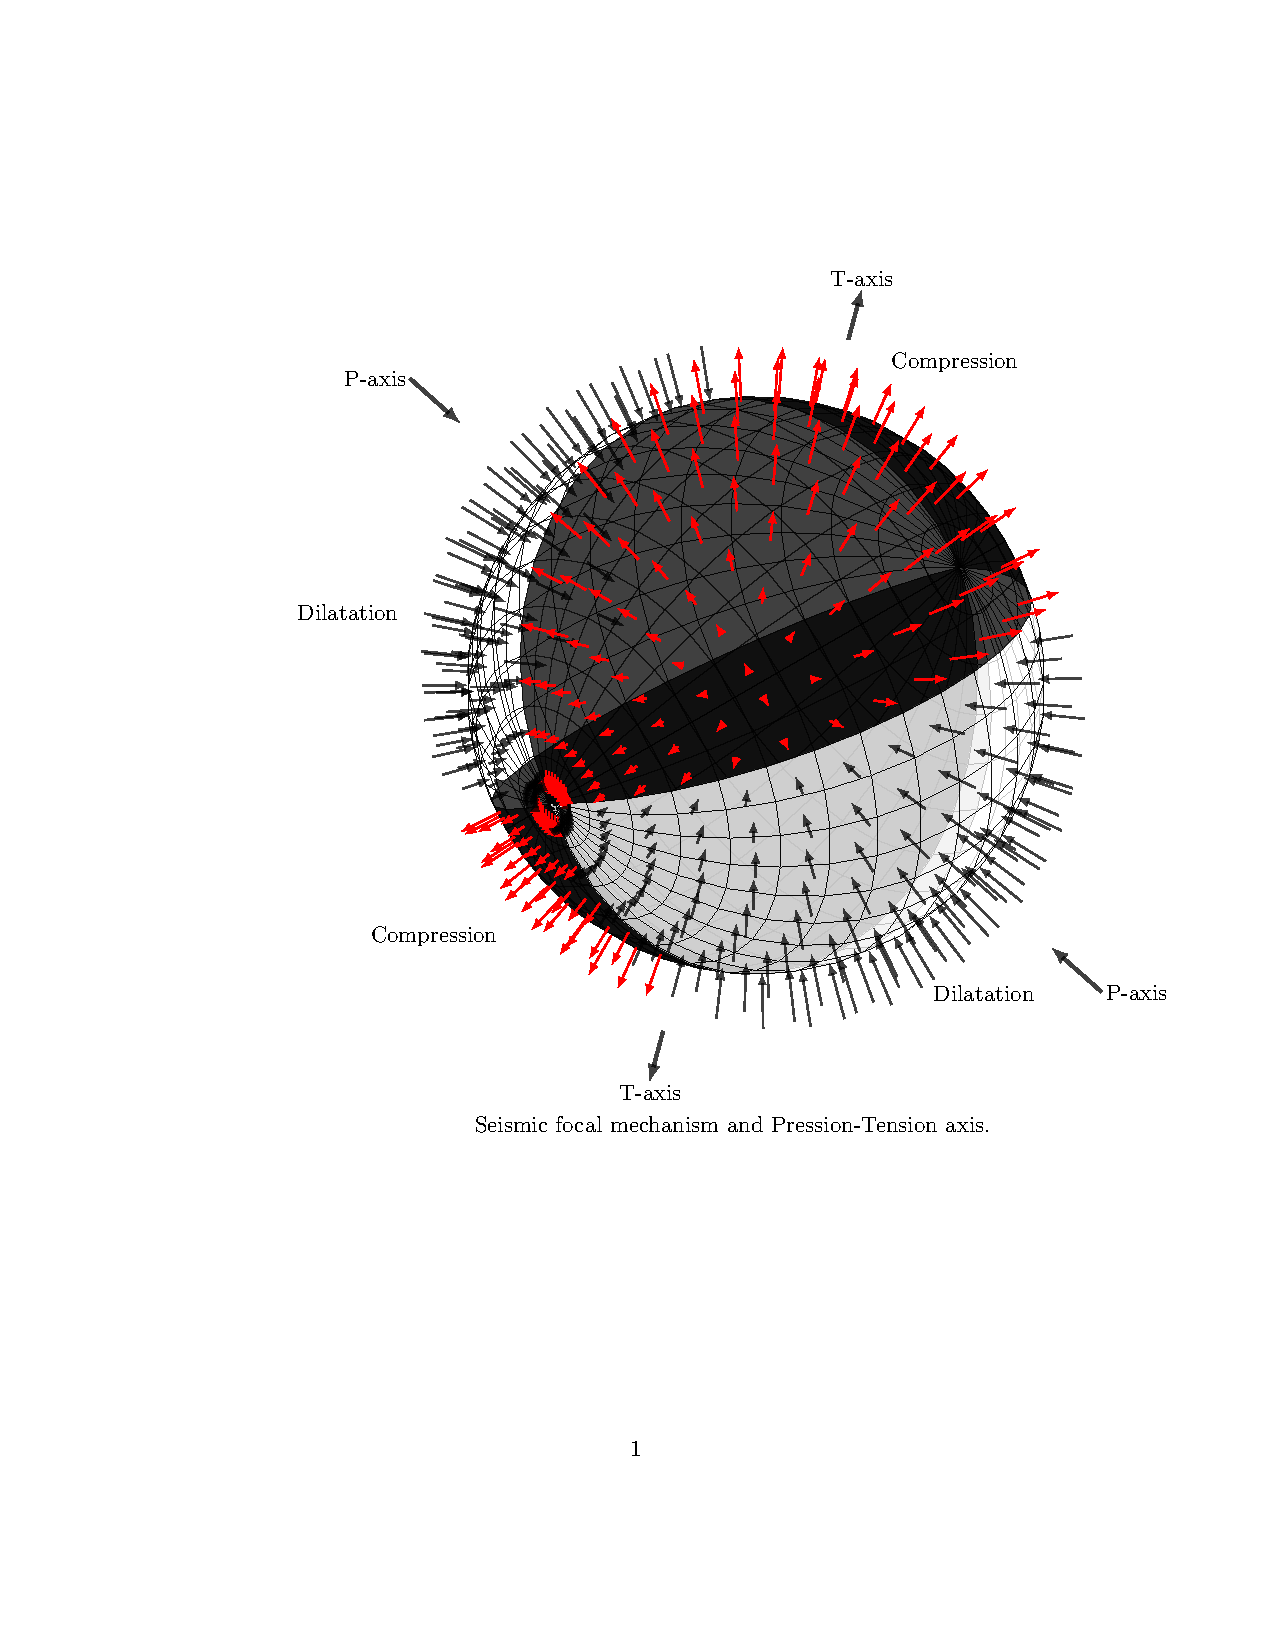
\includegraphics[width=120mm]{SeismicSphere.pdf}
%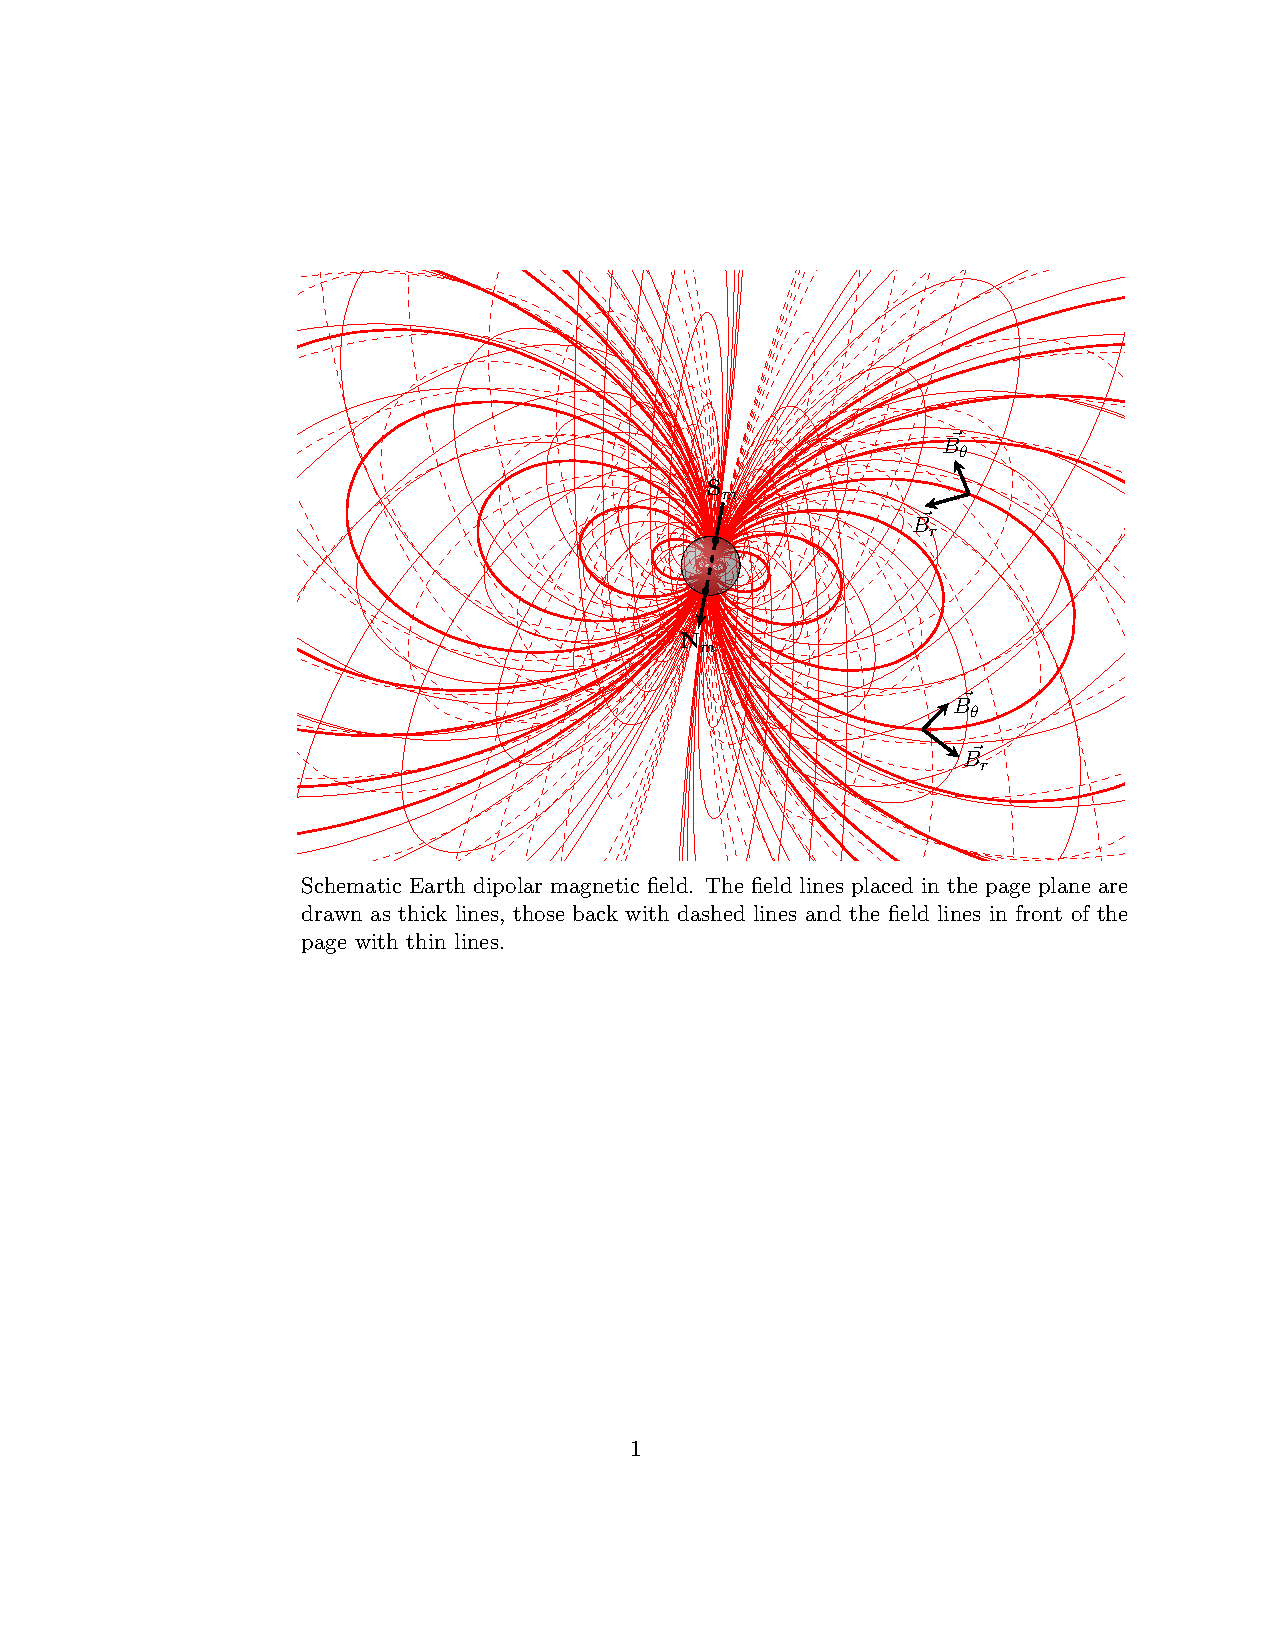
\includepdf[width=50mm]{Magneticfield.pdf}

%\subsubsection{TimeTable}
%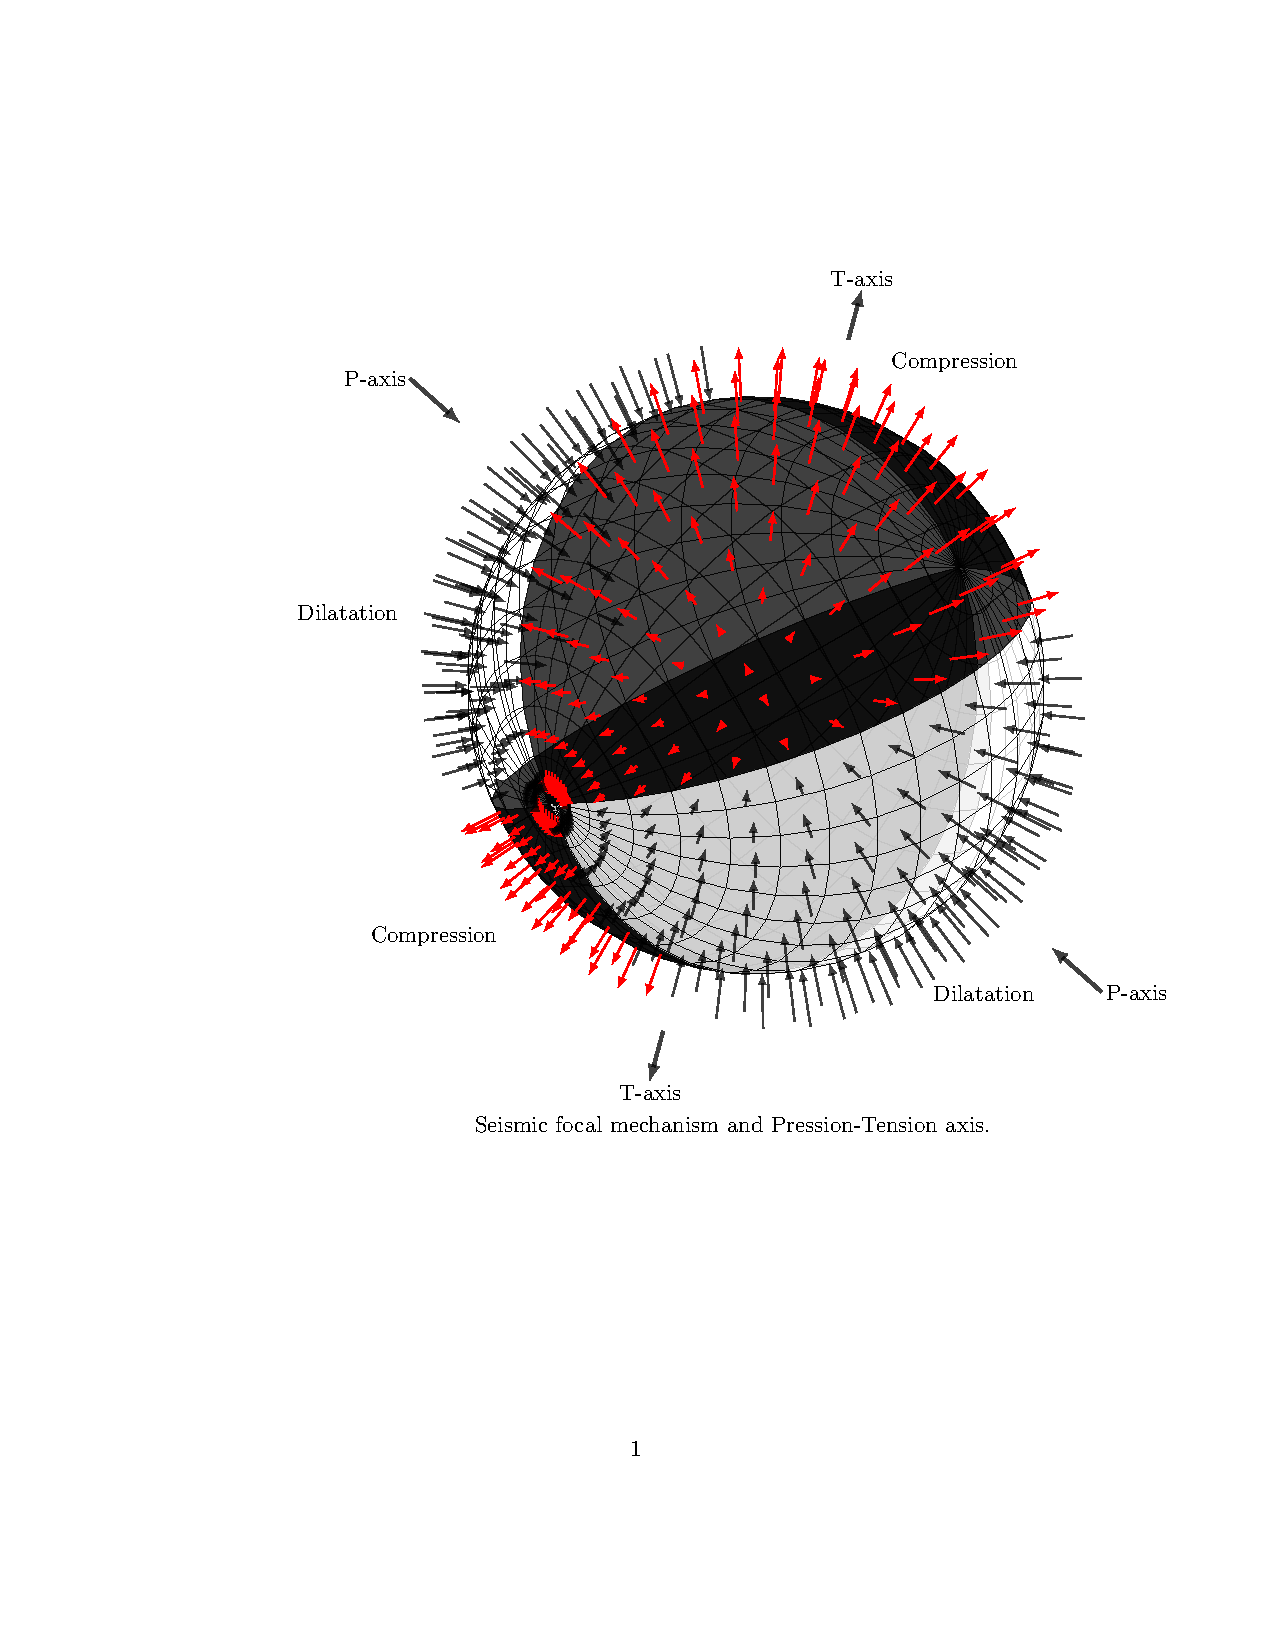
\includegraphics[width=120mm]{SeismicSphere.pdf}
%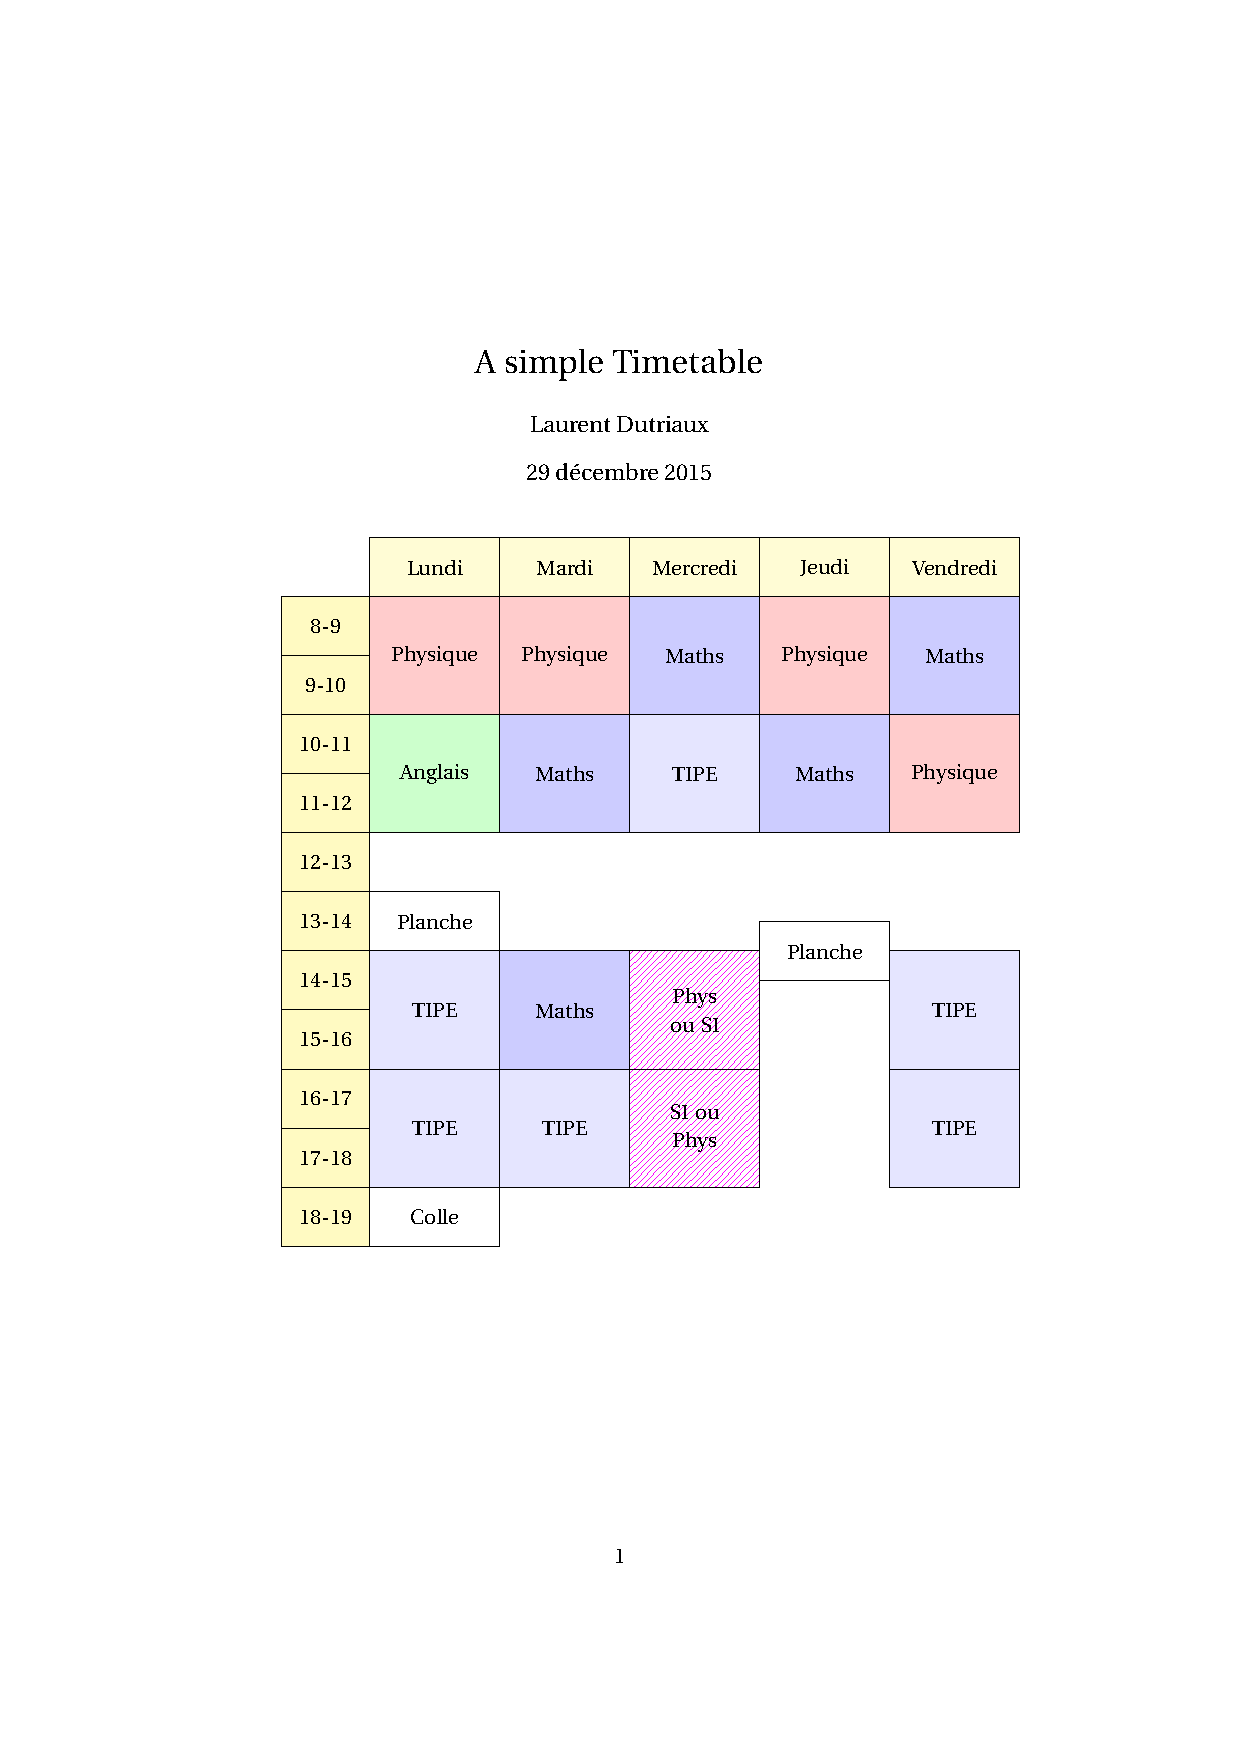
\includepdf[width=50mm]{TimeTable.pdf}

%\subsubsection{Journal de Bord}
%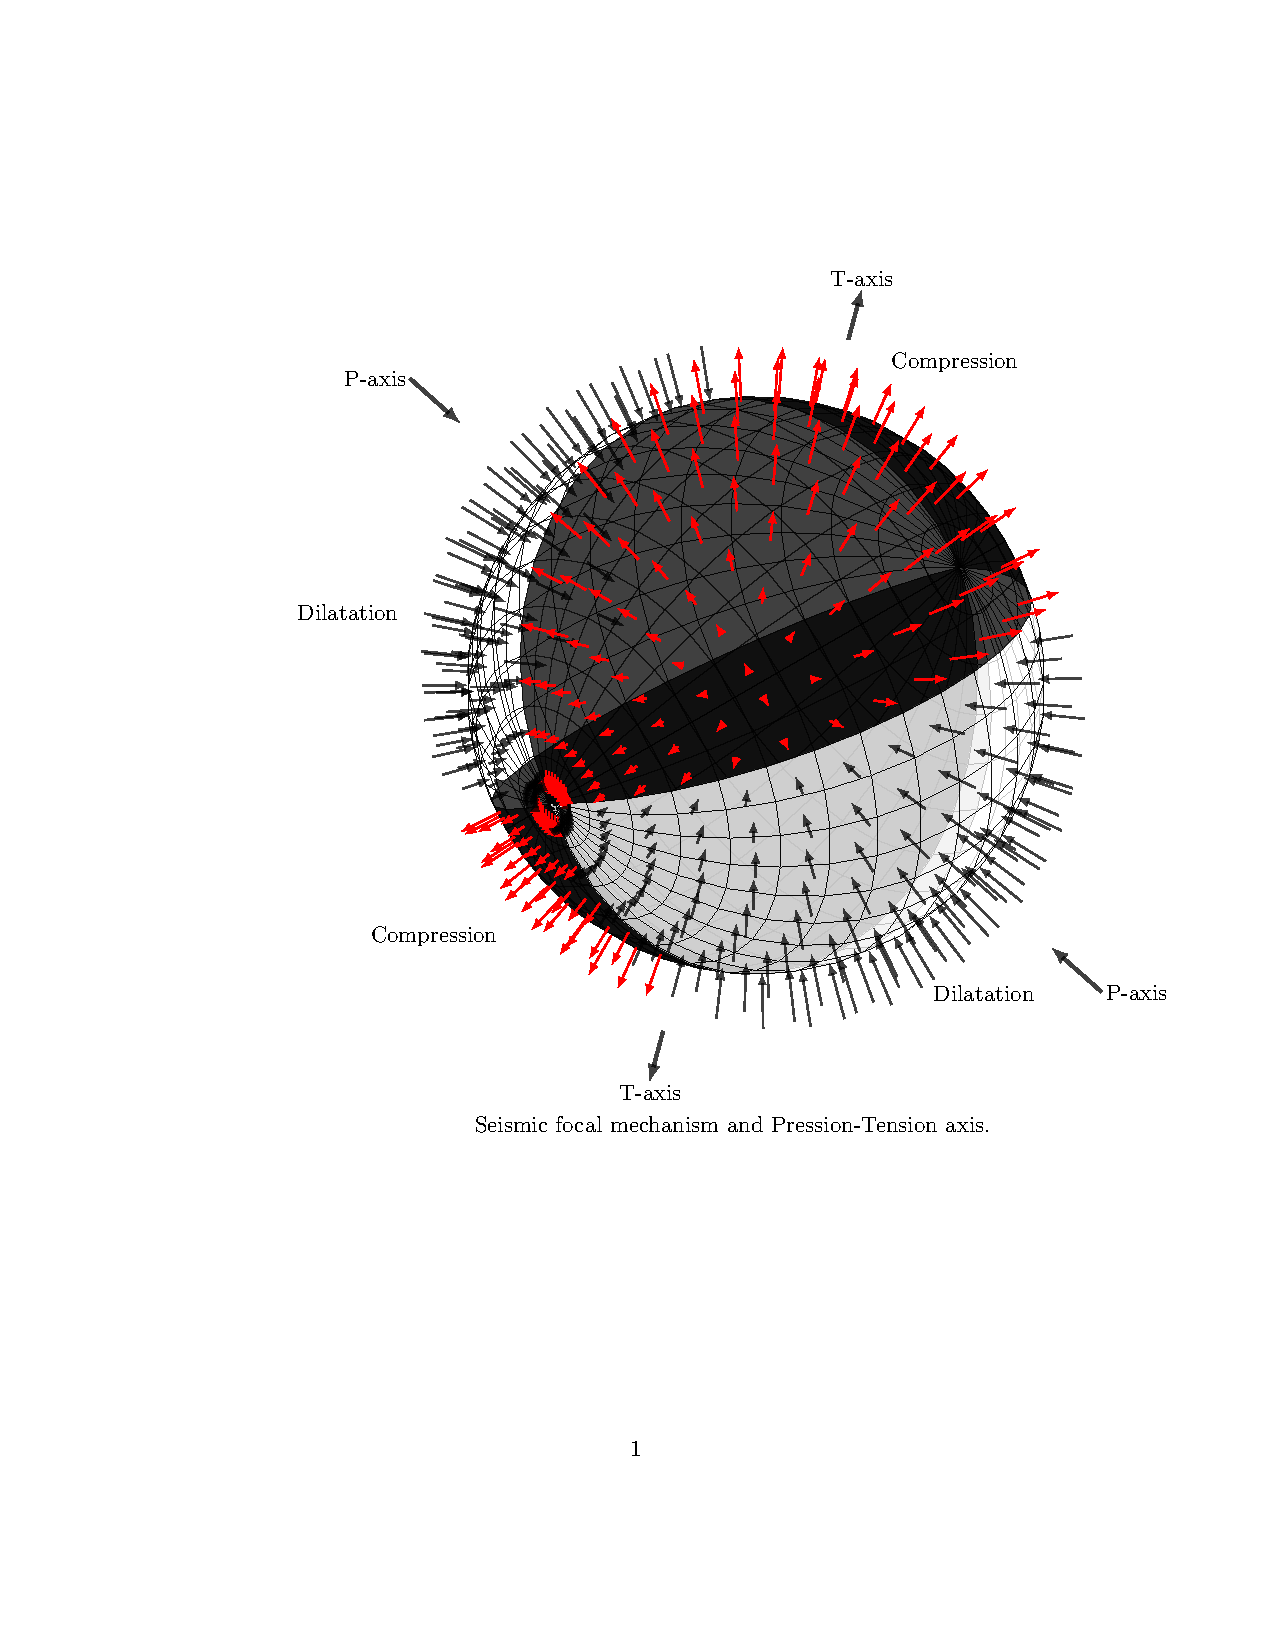
\includegraphics[width=120mm]{SeismicSphere.pdf}
%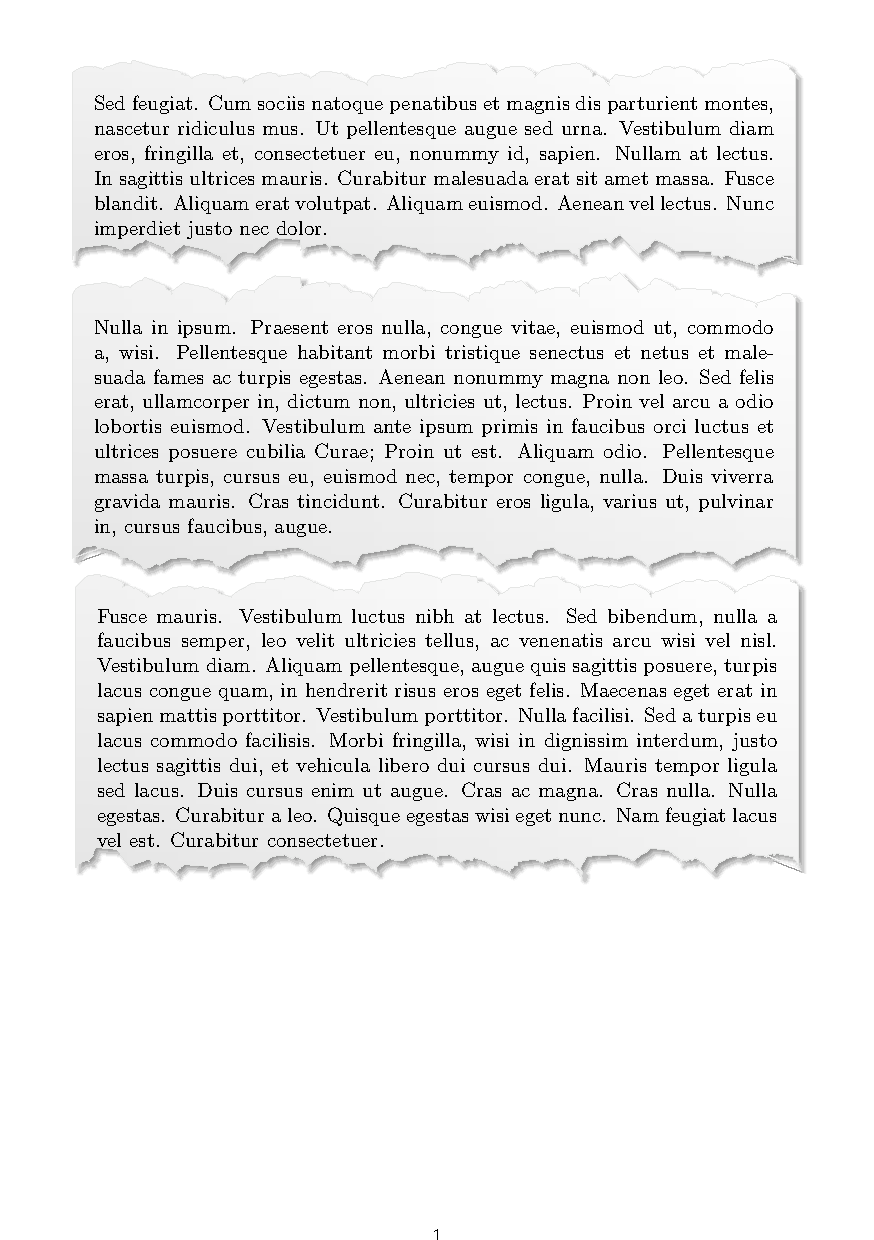
\includepdf[width=50mm]{TornPaper.pdf}

%\subsubsection{Journal de Bord}
%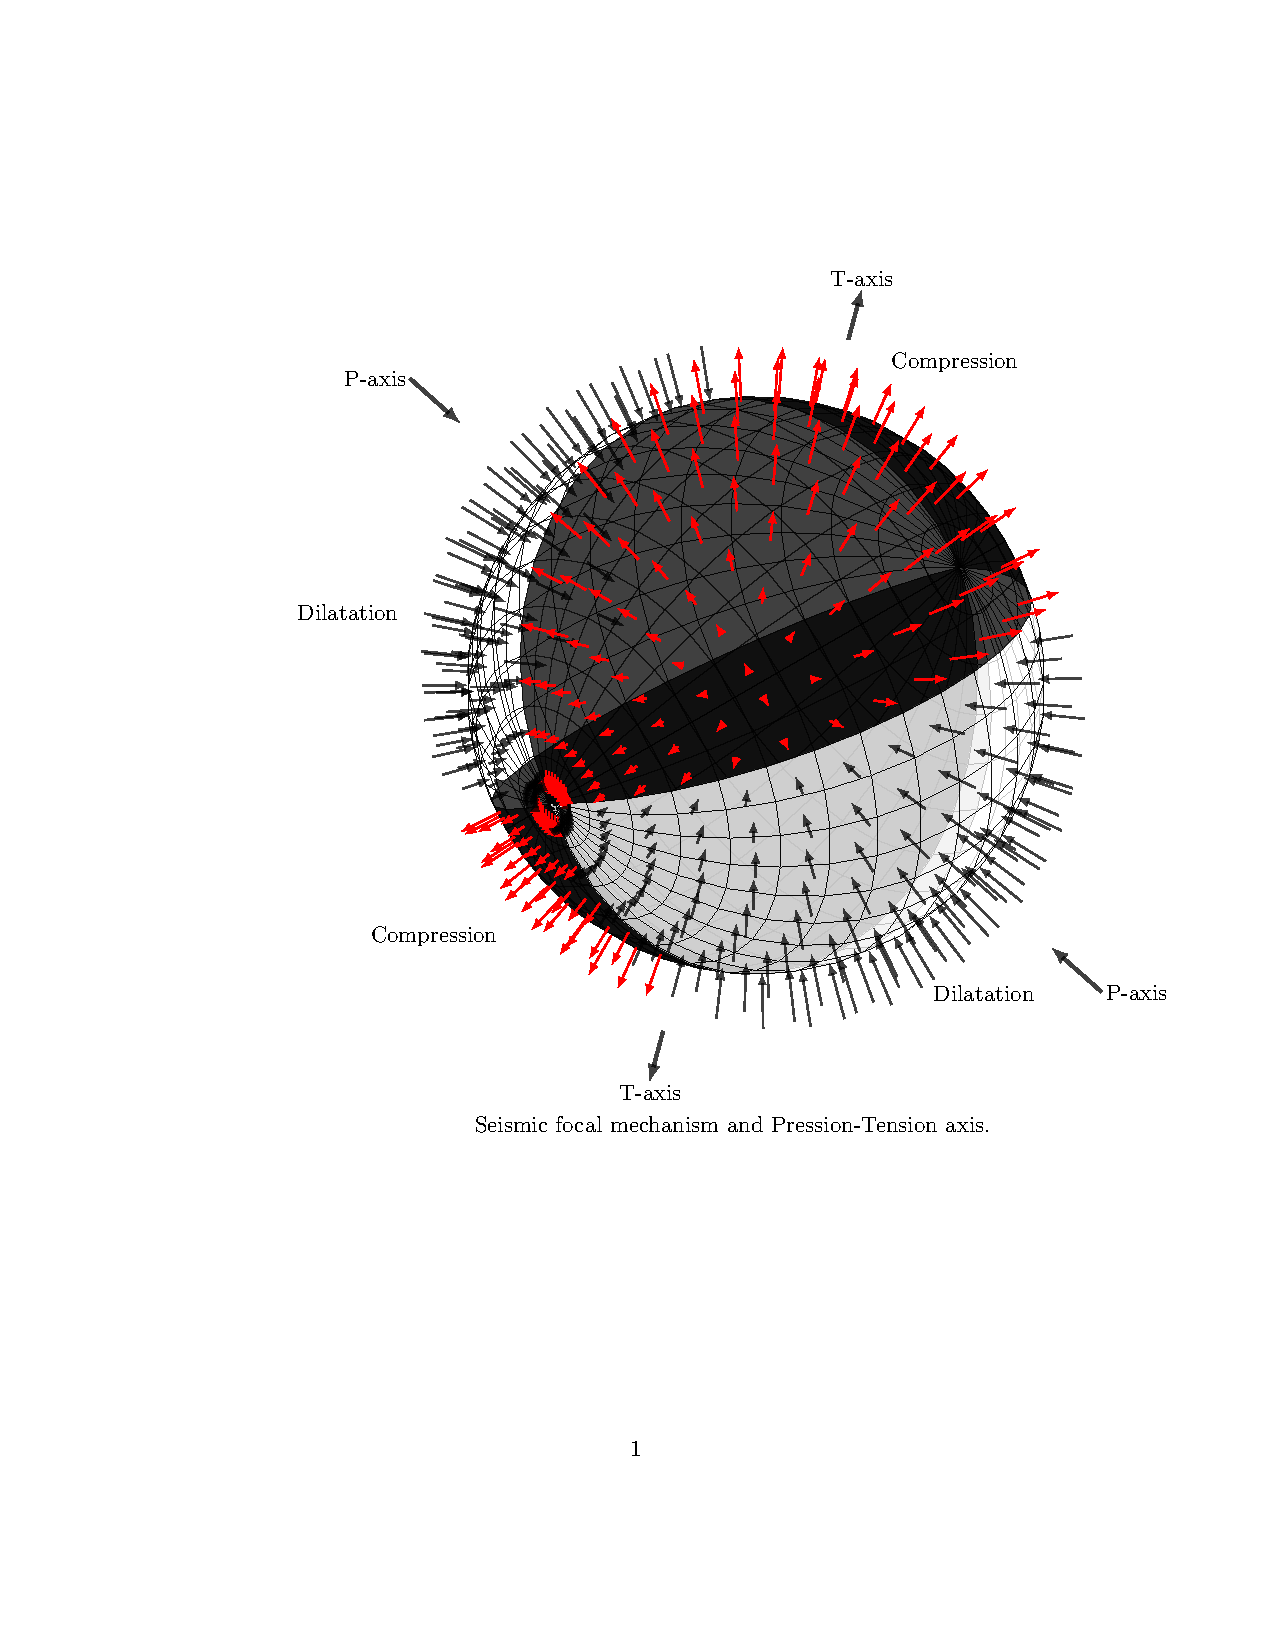
\includegraphics[width=120mm]{SeismicSphere.pdf}
%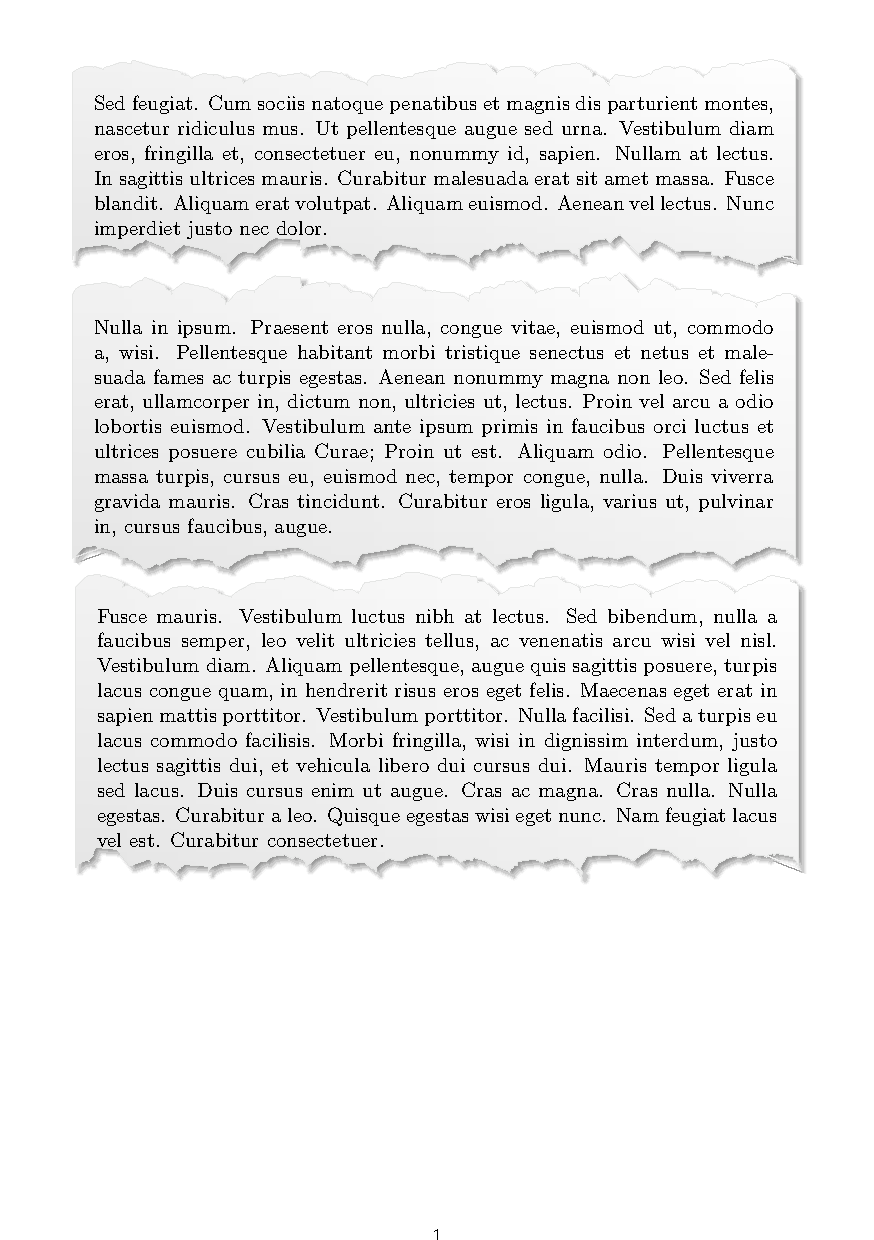
\includepdf{TornPaper.pdf}

\begin{document}
\subsection{Weekly calendar}

%{\footnote
%Pour tous les items il faudrait un mail de rappel comme pour les livrables, meetings et vacances
%}

\begin{calendar}{\hsize}

%----------------------------------------------------------------------------------------
%	FIRST DAY
%----------------------------------------------------------------------------------------

\day{}{
}

% By default all daily events are centered in the box, in order to bring them up use \vspace{2cm} after the event text; you may need to change the 2cm

%----------------------------------------------------------------------------------------
%	SECOND DAY
%----------------------------------------------------------------------------------------

\day{}{
\textbf{9am-10am} \daysep Preparation cours de math \\[3pt]
\textbf{10am-12am} \daysep Preparation presentation finance \\[3pt]
\textbf{1pm-2pm} \daysep Manage my weekly \\[3pt]
\textbf{2pm-4pm} \daysep Administration \\[3pt]
\textbf{4pm-5pm} \daysep Lessive \\[3pt]
\textbf{7pm-10pm} \daysep Cinema \\[3pt]
%\textbf{9am-10am} \daysep BIOSCI101 - BLT100 \\[3pt]
%\textbf{10am-11am} \daysep BIOSCI 104 - LLT \\[3pt]
%\textbf{11am-12pm} \daysep No Lecture \\[3pt]
%\textbf{12pm-1pm} \daysep No Lecture \\[3pt]
%\textbf{12pm-1pm} \daysep BIOSCI105 - BLT204 \\[3pt]
%\textbf{1pm-2pm} \daysep No Lecture \\[3pt]
%\textbf{3pm-4pm} \daysep BIOSCI101 Laboratory \\[3pt]
%\textbf{4pm-5pm} \daysep BIOSCI101 Laboratory
} 

%----------------------------------------------------------------------------------------
%	THIRD DAY
%----------------------------------------------------------------------------------------

\day{}{ % Tuesday
\textbf{9am-10am} \daysep Preparation cours de math \\[3pt]
\textbf{10am-12am} \daysep Preparation presentation finance \\[3pt]
\textbf{10am-12am} \daysep Bibliotheque \\[3pt]
\textbf{10am-12am} \daysep Validation of finances\\[3pt]
\textbf{7pm-9pm} \daysep Krav maga \\[3pt]
%\textbf{3pm-4pm} \daysep No Lecture \\[3pt]
%\textbf{4pm-5pm} \daysep No Lecture
} 

%----------------------------------------------------------------------------------------
%	FOURTH DAY
%----------------------------------------------------------------------------------------

\day{}{ % Wednesday
\textbf{9am-10am} \daysep Preparation cours de math \\[3pt]
\textbf{10am-12am} \daysep Preparation presentation finance \\[3pt]
%\textbf{9am-10am} \daysep No Lecture \\[3pt]
%\textbf{10am-11am} \daysep BIOSCI 104 - LLT \\[3pt]
%\textbf{11am-12pm} \daysep No Lecture \\[3pt]
%\textbf{12pm-1pm} \daysep BIOSCI105 - BLT204 \\[3pt]
%\textbf{1pm-2pm} \daysep No Lecture \\[3pt]
%\textbf{2pm-3pm} \daysep GEO101 - HSB1 \\[3pt]
\textbf{7pm-10pm} \daysep Football \\[3pt]
%\textbf{3pm-4pm} \daysep No Lecture \\[3pt]
%\textbf{4pm-5pm} \daysep No Lecture
} 

%----------------------------------------------------------------------------------------
%	FIFTH DAY
%----------------------------------------------------------------------------------------

\day{}{ % Thursday
\textbf{9am-10am} \daysep Preparation cours de math \\[3pt]
\textbf{10am-12am} \daysep Preparation presentation finance \\[3pt]
\textbf{7pm-9pm} \daysep Krav maga \\[3pt]
%\textbf{9am-10am} \daysep No Lecture \\[3pt]
%\textbf{10am-11am} \daysep BIOSCI 104 - LLT \\[3pt]
%\textbf{11am-12pm} \daysep No Lecture \\[3pt]
%\textbf{12pm-1pm} \daysep No Lecture \\[3pt]
%\textbf{1pm-2pm} \daysep No Lecture \\[3pt]
%\textbf{2pm-3pm} \daysep GEO101 - HSB1 \\[3pt]
%\textbf{3pm-4pm} \daysep No Lecture \\[3pt]
%\textbf{4pm-5pm} \daysep No Lecture
} 

%----------------------------------------------------------------------------------------
%	SIXTH DAY
%----------------------------------------------------------------------------------------

\day{}{ % Friday
\textbf{9am-10am} \daysep Preparation cours de math \\[3pt]
\textbf{10am-12am} \daysep Preparation presentation finance \\[3pt]
\textbf{12am-2pm} \daysep Badminton \\[3pt]
\textbf{9pm-11pm} \daysep Drinks \\[3pt]
%\textbf{10am-11am} \daysep BIOSCI 104 - LLT \\[3pt]
%\textbf{11am-12pm} \daysep No Lecture \\[3pt]
%\textbf{12pm-1pm} \daysep BIOSCI105 - BLT204 \\[3pt]
%\textbf{1pm-2pm} \daysep No Lecture \\[3pt]
%\textbf{2pm-3pm} \daysep No Lecture \\[3pt]
%\textbf{3pm-4pm} \daysep GEO101 Tutorial \\ Room A \\[3pt]
%\textbf{4pm-5pm} \daysep No Lecture
} 

%----------------------------------------------------------------------------------------
%	SEVENTH DAY
%----------------------------------------------------------------------------------------

\day{}{ % Saturday
\textbf{9am-10am} \daysep Preparation cours de math \\[3pt]
\textbf{10am-12am} \daysep Courses \\[3pt]
\textbf{2pm-4pm} \daysep Menage \\[3pt]
\textbf{4pm-9pm} \daysep Get back energy \\[3pt]
\textbf{9pm-11pm} \daysep Go dancing \\[3pt]
\textbf{9pm-11pm} \daysep Go sailing \\[3pt]
}
%----------------------------------------------------------------------------------------
 
\finishCalendar
\end{calendar}

\end{document}
